\documentclass[10pt,journal,compsoc,onecolumn]{IEEEtran}
\usepackage[utf8]{inputenc}
\usepackage{amsmath,amsfonts,amssymb}
\usepackage{amsthm}
\usepackage{graphicx}
\usepackage{cite}
\usepackage{textcomp}
\usepackage{tikz}
\usetikzlibrary{arrows,positioning,shapes.geometric}
\usepackage{booktabs}
\usepackage{url}

\newtheorem{theorem}{Theorem}
\newtheorem{lemma}[theorem]{Lemma}
\newtheorem{definition}[theorem]{Definition}
\newtheorem{corollary}[theorem]{Corollary}

\begin{document}

\title{Algorithmic Foundations of Searching: Monotonic Space Halving, Duplicate Boundary Resolution, Topographical Extremum Traversal, and Discrete Answer Spaces}

\IEEEtitleabstractindextext{%
\begin{abstract}
A comprehensive, pedagogical, and systems-focused engineering masterclass on search algorithms and binary search paradigms. Demystifying logarithmic-time state space exploration without intimidating mathematical recurrences, this paper grounds search mechanics in physical analogies: contrasting the linear scan of an unsorted newspaper with the logarithmic halving of an alphabetized dictionary. We formalize the three universal pillars of binary search (target entity, bounded search space, and monotonic pruning invariants) and address production engineering considerations, including the elimination of 32-bit midpoint integer overflow. We systematically resolve duplicate element clustering via the Answer Variable Pattern, demonstrating how first- and last-occurrence boundary detection enables instantaneous O(log N) frequency counting in chronological telemetry databases. Dispelling the widespread misconception that binary search requires globally sorted arrays, we prove how local geometric slopes guarantee valley descent to a local minimum in unsorted collections with distinct elements. Finally, we generalize binary search to implicit mathematical answer spaces, computing integer square roots through monotonic boolean predicate transitions. Complete, compilable Java implementations and diagnostic dry-run tables accompany all discussed algorithms.
\end{abstract}

\begin{IEEEkeywords}
Binary Search, search space halving, monotonic invariants, first occurrence, last occurrence, local minima, peak finding, answer space search, integer square root, algorithm analysis
\end{IEEEkeywords}
}

\maketitle
\IEEEdisplaynontitleabstractindextext
\IEEEpeerreviewmaketitle

\section{Introduction: The Search Paradigm and the Cost of Unordered Information}
\label{sec:intro}

Searching is among the most frequent and mission-critical computational operations in computer systems. From querying index records in distributed databases and scanning chronological server telemetry logs to routing packets across routing tables, locating a target value efficiently dictates whether a system responds in microseconds or grinds to a halt.

To understand why searching algorithms are structured the way they are, consider the physical comparison introduced in technical computer science lectures:
\begin{itemize}
    \item \textbf{Searching a Word in a Newspaper (Linear Search):} A newspaper article is an unsorted collection of words. If a reader wishes to verify whether a specific word appears, there is no structural clue indicating where the word might reside. In the worst case, the reader must inspect all 240,000 words printed on the pages sequentially. If the document contains $N$ words, this brute-force approach requires $O(N)$ operations.
    \item \textbf{Searching a Word in an Oxford Dictionary (Binary Search):} A dictionary is sorted alphabetically from A to Z. A reader never starts on page 1 scanning word by word. Instead, the reader opens the dictionary roughly in the middle. By comparing the target word with the words on the current page, the reader makes a decisive deduction:
    \begin{itemize}
        \item If the target word alphabetically precedes the current page, the entire right half of the book (thousands of pages) is permanently discarded.
        \item If the target word succeeds the current page, the entire left half is discarded.
    \end{itemize}
\end{itemize}

\subsection{The Power of Logarithmic Halving}

By discarding exactly half of the remaining candidate space in every step, the search space collapses with astonishing speed:
\[
240{,}000 \longrightarrow 120{,}000 \longrightarrow 60{,}000 \longrightarrow 30{,}000 \longrightarrow 15{,}000 \longrightarrow 7{,}500 \longrightarrow 3{,}750 \longrightarrow \dots \longrightarrow 1
\]
On an unsorted collection of 240,000 words, linear search requires up to 240,000 comparisons. In sharp contrast, binary search resolves the lookup in at most $\lceil \log_2(240{,}000) \rceil = 18$ comparisons! 

This exponential speedup transforms impractical workloads into real-time sub-millisecond computations.

\subsection{The Three Universal Pillars of Binary Search}

Contrary to common belief among novice engineers, binary search is not merely an array lookup routine. It is a universal algorithmic strategy applicable whenever a problem satisfies three core pillars:
\begin{enumerate}
    \item \textbf{Target:} A well-defined value, boundary, or condition to be discovered.
    \item \textbf{Search Space:} A bounded range $[l, r]$ containing all possible candidate positions or values.
    \item \textbf{Reduction Condition (Pruning Invariant):} A verifiable property that guarantees which half of the search space can be safely discarded without losing the target.
\end{enumerate}

In this paper, we explore how these three pillars govern canonical lookups, duplicate-handling variants, local extrema in unsorted collections, and monotonic answer spaces.

% -----------------------------------------------------------------------------
\section{Canonical Binary Search on Sorted Arrays}
\label{sec:canonical}

\subsection{Problem Formulation}

Given an array of $N$ integers sorted in non-decreasing order and a target value $K$, determine the 0-based index of $K$ in the array. If $K$ is not present, return $-1$.

\subsection{Pointer Mechanics and Invariant Boundaries}

Binary search establishes two pointers defining the active search space window:
\begin{itemize}
    \item $l = 0$ (the inclusive left boundary).
    \item $r = N - 1$ (the inclusive right boundary).
\end{itemize}

In each iteration, we calculate the midpoint index $mid$. We then evaluate three mutually exclusive cases:
\begin{enumerate}
    \item \textbf{Exact Match ($A[mid] == K$):} Target located. Return $mid$ immediately.
    \item \textbf{Target is Larger ($A[mid] < K$):} Because the array is sorted, every element from index $l$ up to $mid$ is strictly less than or equal to $A[mid]$, and therefore strictly less than $K$. No solution can exist in the left half $[l \dots mid]$. We prune it by setting $l = mid + 1$.
    \item \textbf{Target is Smaller ($A[mid] > K$):} Every element from index $mid$ to $r$ is strictly greater than $K$. No solution can exist in the right half $[mid \dots r]$. We prune it by setting $r = mid - 1$.
\end{enumerate}

\subsection{Critical Systems Consideration: Midpoint Overflow}

A subtle bug present in early standard library implementations is the computation of the midpoint:
\begin{verbatim}
int mid = (l + r) / 2; // DANGEROUS: Potential 32-bit Integer Overflow!
\end{verbatim}
When $l$ and $r$ are large (e.g., $l + r > 2^{31} - 1 \approx 2.14 \times 10^9$), their sum overflows into a negative 32-bit integer, resulting in a negative index and an immediate memory fault or \texttt{ArrayIndexOutOfBoundsException}.

The safe, production-grade calculation distributes the division:
\begin{verbatim}
int mid = l + (r - l) / 2; // SAFE: Arithmetic cannot overflow
\end{verbatim}

\begin{figure}[h]
\centering
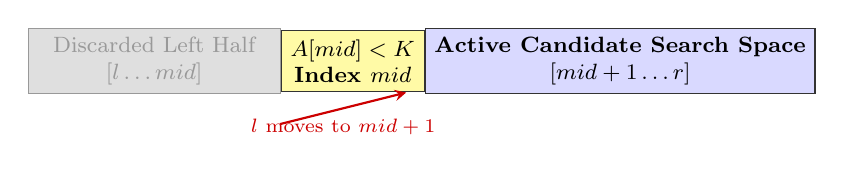
\begin{tikzpicture}[
    box/.style={rectangle, draw=black!80, font=\footnotesize, align=center, minimum height=0.75cm},
    elim/.style={rectangle, draw=black!40, fill=gray!25, text=black!40, font=\footnotesize, align=center, minimum height=0.75cm},
    active/.style={rectangle, draw=black!80, fill=blue!15, font=\footnotesize\bfseries, align=center, minimum height=0.75cm},
    midpt/.style={rectangle, draw=black!80, fill=yellow!35, font=\footnotesize\bfseries, align=center, minimum height=0.75cm},
    arrow/.style={-stealth, thick, red!80!black}
]
\node[elim, minimum width=3.2cm] (left_elim) at (0,0) {Discarded Left Half\\$[l \dots mid]$};
\node[midpt, minimum width=1.6cm, right=0.0cm of left_elim] (m) {$A[mid] < K$\\Index $mid$};
\node[active, minimum width=3.8cm, right=0.0cm of m] (right_act) {Active Candidate Search Space\\$[mid + 1 \dots r]$};

\draw[arrow] (1.6, -0.8) -- node[below, font=\scriptsize] {$l$ moves to $mid + 1$} (3.2, -0.4);
\end{tikzpicture}
\caption{Binary Search Search-Space Halving: Discarding the Left Half when $A[mid] < K$.}
\label{fig:bs_halving}
\end{figure}

\subsection{Diagnostic Walkthrough on Lecture Example}

Consider the 10-element sorted array from page 4 of the lecture notes:
\begin{verbatim}
Index:    0   1   2    3    4    5    6    7    8    9
Array: [  3,  6,  9,  12,  14,  19,  20,  23,  25,  27 ]
\end{verbatim}

\subsubsection{Trace 1: Searching for Target $K = 20$}
\begin{itemize}
    \item \textbf{Pass 1:} $l = 0$, $r = 9$.
    \[
    mid = 0 + (9 - 0) / 2 = 4 \implies A[4] = 14
    \]
    Since $A[4] = 14 < 20$, target must be in the right half. Set $l = mid + 1 = 5$.
    \item \textbf{Pass 2:} $l = 5$, $r = 9$.
    \[
    mid = 5 + (9 - 5) / 2 = 7 \implies A[7] = 23
    \]
    Since $A[7] = 23 > 20$, target must be in the left half. Set $r = mid - 1 = 6$.
    \item \textbf{Pass 3:} $l = 5$, $r = 6$.
    \[
    mid = 5 + (6 - 5) / 2 = 5 \implies A[5] = 19
    \]
    Since $A[5] = 19 < 20$, target must be in the right half. Set $l = mid + 1 = 6$.
    \item \textbf{Pass 4:} $l = 6$, $r = 6$.
    \[
    mid = 6 + (6 - 6) / 2 = 6 \implies A[6] = 20
    \]
    Since $A[6] == 20$, target match found! Return index $6$.
\end{itemize}

\subsubsection{Trace 2: Searching for Absent Target $K = 15$}
\begin{itemize}
    \item \textbf{Pass 1:} $l = 0, r = 9, mid = 4 \implies A[4] = 14 < 15 \implies l = 5$.
    \item \textbf{Pass 2:} $l = 5, r = 9, mid = 7 \implies A[7] = 23 > 15 \implies r = 6$.
    \item \textbf{Pass 3:} $l = 5, r = 6, mid = 5 \implies A[5] = 19 > 15 \implies r = 4$.
    \item \textbf{Termination:} Now $l = 5$ and $r = 4$. Because $l > r$, the search space is exhausted. Return $-1$.
\end{itemize}

\subsection{Reference Implementation}

\begin{verbatim}
public class BinarySearchEngine {
    public static int search(int[] A, int K) {
        if (A == null || A.length == 0) return -1;

        int l = 0;
        int r = A.length - 1;

        while (l <= r) {
            int mid = l + (r - l) / 2;

            if (A[mid] == K) {
                return mid; // Target found
            } else if (A[mid] < K) {
                l = mid + 1; // Search right half
            } else {
                r = mid - 1; // Search left half
            }
        }
        return -1; // Target absent
    }
}
\end{verbatim}

\textbf{Complexity Analysis:}
\begin{itemize}
    \item \textbf{Time Complexity:} $O(\log N)$. With each step, the search space $N$ is halved: $N, N/2, N/4, \dots, 1$.
    \item \textbf{Auxiliary Space Complexity:} $O(1)$. Execution requires only three integer pointer variables.
\end{itemize}

% -----------------------------------------------------------------------------
\section{Handling Duplicates: First and Last Occurrences via the Answer Variable Pattern}
\label{sec:duplicates}

\subsection{The Enterprise Motivation: Chronological Telemetry and Logs}

In enterprise infrastructure (illustrated on page 9 of the lecture notes), logs or emails are stored sorted by date or year:
\begin{verbatim}
Year:    2023, 2023, 2023, ..., 2024, 2024, 2024, ..., 2025, 2026
Record:  Log-1 Log-2 Log-3 ...  Log-K Log-K+1 ...      ...
\end{verbatim}
A typical operational inquiry is: \textbf{``Find the very first email or log entry generated in the year 2024.''}

If we execute canonical binary search and land on a record with year $2024$, returning immediately is incorrect. That record might be the 500th entry of that year. We need the \textbf{first occurrence}.

\subsection{The Rookie Trap vs. The Answer Variable Pattern}

\begin{itemize}
    \item \textbf{The Rookie Approach ($O(N)$ Degraded):} Run canonical binary search until finding any match, then perform a linear scan leftward until hitting a different value. If all elements in the array are duplicates of $K$ (e.g., $10^5$ copies of 5), the linear scan degrades the algorithm to $O(N)$, defeating the purpose of binary search.
    \item \textbf{The Senior Approach ($O(\log N)$ Guaranteed):} \textbf{The Answer Variable Pattern.}
    \begin{enumerate}
        \item Allocate an integer \texttt{ans = -1}.
        \item When $A[mid] == K$, do not terminate. Record \texttt{ans = mid} as a valid candidate.
        \item Because a potentially earlier occurrence can only exist to the left, aggressively prune the right half by setting \texttt{r = mid - 1}!
        \item Allow the \verb|while (l <= r)| loop to run until natural exhaustion.
    \end{enumerate}
\end{itemize}

\begin{figure}[h]
\centering
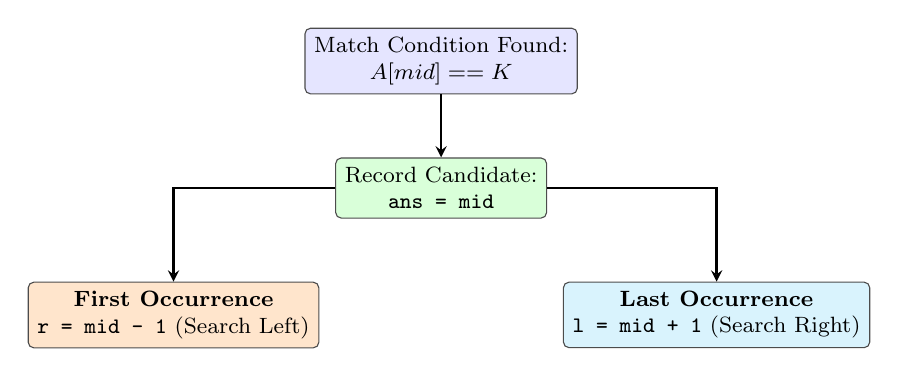
\begin{tikzpicture}[
    box/.style={rectangle, draw=black!70, fill=blue!10, rounded corners=2pt, font=\footnotesize, align=center, minimum height=0.7cm, minimum width=2.4cm},
    action/.style={rectangle, draw=black!70, rounded corners=2pt, font=\footnotesize, align=center, minimum height=0.7cm, minimum width=2.6cm},
    arrow/.style={-stealth, thick}
]
\node[box] (match) at (0,0) {Match Condition Found:\\$A[mid] == K$};
\node[action, fill=green!15, below=0.8cm of match] (store) {Record Candidate:\\\texttt{ans = mid}};
\node[action, fill=orange!20, below left=0.8cm and 0.2cm of store] (first_occ) {\textbf{First Occurrence}\\\texttt{r = mid - 1} (Search Left)};
\node[action, fill=cyan!15, below right=0.8cm and 0.2cm of store] (last_occ) {\textbf{Last Occurrence}\\\texttt{l = mid + 1} (Search Right)};

\draw[arrow] (match) -- (store);
\draw[arrow] (store) -| (first_occ);
\draw[arrow] (store) -| (last_occ);
\end{tikzpicture}
\caption{The Answer Variable Pattern for Boundary Searches on Duplicate Clusters.}
\label{fig:ans_pattern}
\end{figure}

\subsection{Detailed Trace of First Occurrence on Lecture Array}

Consider the 15-element duplicate array from page 10 of the lecture notes:
\begin{verbatim}
Index:   0   1   2   3  4  5  6  7  8  9  10 11 12  13  14
Array: [-5, -5, -3,  0, 0, 1, 5, 5, 5, 5,  5, 8, 10, 10, 15 ]
\end{verbatim}
We seek the first occurrence of $K = 5$. The duplicates of 5 span indices $[6 \dots 10]$. The expected answer is index $6$.

\begin{table}[h]
\centering
\caption{Step-by-Step Execution Table: First Occurrence of $K = 5$}
\label{tab:first_occurrence_trace}
\begin{tabular}{@{}cccclc@{}}
\toprule
\textbf{Step} & $l$ & $r$ & $mid$ & \textbf{Evaluation \& State Action} & \texttt{ans} \\ \midrule
\textbf{1} & $0$ & $14$ & $7$ & $A[7] == 5$: Valid match. Store \texttt{ans = 7}. Search left: $r = 7 - 1 = 6$. & $7$ \\
\textbf{2} & $0$ & $6$ & $3$ & $A[3] = 0 < 5$: Value too small. Search right: $l = 3 + 1 = 4$. & $7$ \\
\textbf{3} & $4$ & $6$ & $5$ & $A[5] = 1 < 5$: Value too small. Search right: $l = 5 + 1 = 6$. & $7$ \\
\textbf{4} & $6$ & $6$ & $6$ & $A[6] == 5$: Valid match. Store \texttt{ans = 6}. Search left: $r = 6 - 1 = 5$. & $6$ \\
\textbf{5} & $6$ & $5$ & -- & $l > r$ ($6 > 5$): Boundary invalid. Loop terminates. & \textbf{6} \\ \bottomrule
\end{tabular}
\end{table}

The algorithm terminates naturally and returns the correct index: \textbf{6}.

\subsection{Extension: Last Occurrence and Frequency Range Counting}

To find the \textbf{last occurrence} of $K$, the logic is symmetric:
\begin{itemize}
    \item When $A[mid] == K$, record \texttt{ans = mid}.
    \item To discover if a later occurrence exists to the right, set \texttt{l = mid + 1}.
\end{itemize}

\textbf{Computing Total Occurrences in $O(\log N)$ Time:}
In database indexing, calculating the total number of records matching key $K$ without scanning every record is a fundamental primitive:
\[
\text{Total Count} = (\text{lastOccurrence}(A, K) - \text{firstOccurrence}(A, K) + 1)
\]
Both calls run in $O(\log N)$, providing an instantaneous frequency count in $O(\log N)$ time and $O(1)$ space.

\subsection{Production Java Implementation: First Occurrence}

\begin{verbatim}
public class DuplicateBinarySearch {
    // Finds the first (lowest index) occurrence of target K
    public static int findFirstOccurrence(int[] A, int K) {
        int l = 0;
        int r = A.length - 1;
        int ans = -1;

        while (l <= r) {
            int mid = l + (r - l) / 2;

            if (A[mid] == K) {
                ans = mid;    // Record valid candidate
                r = mid - 1;  // Continue searching leftward
            } else if (A[mid] < K) {
                l = mid + 1;  // Search rightward
            } else {
                r = mid - 1;  // Search leftward
            }
        }
        return ans;
    }

    // Finds the last (highest index) occurrence of target K
    public static int findLastOccurrence(int[] A, int K) {
        int l = 0;
        int r = A.length - 1;
        int ans = -1;

        while (l <= r) {
            int mid = l + (r - l) / 2;

            if (A[mid] == K) {
                ans = mid;    // Record valid candidate
                l = mid + 1;  // Continue searching rightward
            } else if (A[mid] < K) {
                l = mid + 1;
            } else {
                r = mid - 1;
            }
        }
        return ans;
    }
}
\end{verbatim}

% -----------------------------------------------------------------------------
\section{Binary Search on Unsorted Arrays: Local Minima and Peak Finding}
\label{sec:local_minima}

One of the most persistent misconceptions among software engineering candidates is the belief that \emph{Binary Search can only be applied to sorted arrays}. This is demonstrably false.

As established in Section~\ref{sec:intro}, Binary Search only requires a \textbf{decision condition} that guarantees which half of the search space contains a solution. Sorting is merely one way to provide such a guarantee.

\subsection{Problem Statement: Finding Any Local Minimum}

Given an array $A$ of $N$ integers where all adjacent elements are distinct ($A[i] \neq A[i+1]$), find \textbf{any one} local minimum. An element is a local minimum if it is strictly smaller than its existing neighbors:
\begin{itemize}
    \item For index $0$: $A[0] < A[1]$.
    \item For index $N - 1$: $A[N - 1] < A[N - 2]$.
    \item For any internal index $i$ ($0 < i < N - 1$): $A[i] < A[i - 1]$ \textbf{and} $A[i] < A[i + 1]$.
\end{itemize}

\subsection{The Mental Model: The Inevitable Valley Descent}

Imagine standing on a rugged terrain of mountains and valleys. If you take a step downhill, and continue stepping downhill whenever possible, can you walk infinitely? 
No, because the array has a finite length and finite values. You are mathematically guaranteed to reach the bottom of a valley—a \textbf{Local Minimum}.

\subsection{The Four Geometric Slope Cases at Midpoint}

When inspecting an internal element $A[mid]$ with its immediate neighbors $A[mid - 1]$ and $A[mid + 1]$, exactly four geometric configurations are possible:

\begin{figure}[h]
\centering
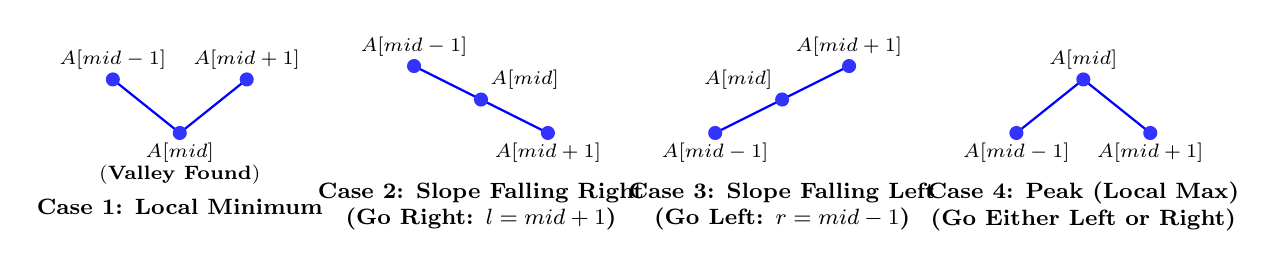
\begin{tikzpicture}[
    scale=0.85,
    pt/.style={circle, fill=blue!80, inner sep=1.8pt},
    lbl/.style={font=\scriptsize, align=center}
]
% Case 1: Valley
\begin{scope}[shift={(0,0)}]
    \draw[thick, blue] (-1, 0.8) -- (0, 0) -- (1, 0.8);
    \node[pt] at (-1, 0.8) {}; \node[lbl, above] at (-1, 0.8) {$A[mid-1]$};
    \node[pt] at (0, 0) {}; \node[lbl, below] at (0, 0) {$A[mid]$\\(\textbf{Valley Found})};
    \node[pt] at (1, 0.8) {}; \node[lbl, above] at (1, 0.8) {$A[mid+1]$};
    \node[lbl, font=\footnotesize\bfseries] at (0, -1.1) {Case 1: Local Minimum};
\end{scope}

% Case 2: Downward slope to right
\begin{scope}[shift={(4.5,0)}]
    \draw[thick, blue] (-1, 1.0) -- (0, 0.5) -- (1, 0);
    \node[pt] at (-1, 1.0) {}; \node[lbl, above] at (-1, 1.0) {$A[mid-1]$};
    \node[pt] at (0, 0.5) {}; \node[lbl, above right] at (0, 0.5) {$A[mid]$};
    \node[pt] at (1, 0) {}; \node[lbl, below] at (1, 0) {$A[mid+1]$};
    \node[lbl, font=\footnotesize\bfseries] at (0, -1.1) {Case 2: Slope Falling Right\\(Go Right: $l = mid + 1$)};
\end{scope}

% Case 3: Upward slope to right
\begin{scope}[shift={(9,0)}]
    \draw[thick, blue] (-1, 0) -- (0, 0.5) -- (1, 1.0);
    \node[pt] at (-1, 0) {}; \node[lbl, below] at (-1, 0) {$A[mid-1]$};
    \node[pt] at (0, 0.5) {}; \node[lbl, above left] at (0, 0.5) {$A[mid]$};
    \node[pt] at (1, 1.0) {}; \node[lbl, above] at (1, 1.0) {$A[mid+1]$};
    \node[lbl, font=\footnotesize\bfseries] at (0, -1.1) {Case 3: Slope Falling Left\\(Go Left: $r = mid - 1$)};
\end{scope}

% Case 4: Peak
\begin{scope}[shift={(13.5,0)}]
    \draw[thick, blue] (-1, 0) -- (0, 0.8) -- (1, 0);
    \node[pt] at (-1, 0) {}; \node[lbl, below] at (-1, 0) {$A[mid-1]$};
    \node[pt] at (0, 0.8) {}; \node[lbl, above] at (0, 0.8) {$A[mid]$};
    \node[pt] at (1, 0) {}; \node[lbl, below] at (1, 0) {$A[mid+1]$};
    \node[lbl, font=\footnotesize\bfseries] at (0, -1.1) {Case 4: Peak (Local Max)\\(Go Either Left or Right)};
\end{scope}
\end{tikzpicture}
\caption{The Four Geometric Topographical Slopes Governing Local Minima Decisions.}
\label{fig:local_minima_slopes}
\end{figure}

\begin{enumerate}
    \item \textbf{Case 1: Valley ($A[mid] < A[mid - 1]$ and $A[mid] < A[mid + 1]$):} The current element is strictly smaller than both neighbors. It is by definition a local minimum. Return $mid$.
    \item \textbf{Case 2: Falling Slope to the Right ($A[mid] > A[mid + 1]$):} The terrain is descending toward the right. Since the boundary at $N - 1$ must eventually bound the descent, a local minimum is \textbf{guaranteed to exist in the right half}. We set $l = mid + 1$.
    \item \textbf{Case 3: Falling Slope to the Left ($A[mid] > A[mid - 1]$):} The terrain is descending toward the left. A local minimum is \textbf{guaranteed to exist in the left half}. We set $r = mid - 1$.
    \item \textbf{Case 4: Peak ($A[mid] > A[mid - 1]$ and $A[mid] > A[mid + 1]$):} The element is a local peak, descending in \textbf{both} directions. Therefore, a valley is guaranteed to exist on \emph{both} the left and right sides! We can greedily discard either side (e.g., $r = mid - 1$).
\end{enumerate}

\subsection{Handling Array Boundaries Cleanly}

To avoid out-of-bounds indexing during neighbor checks ($mid - 1$ and $mid + 1$), we employ the clean engineering pattern taught in the lecture (page 20):
\begin{enumerate}
    \item Handle arrays of length $N = 1$ trivially (index $0$ is the minimum).
    \item Check boundary index $0$: If $A[0] < A[1]$, return index $0$.
    \item Check boundary index $N - 1$: If $A[N - 1] < A[N - 2]$, return index $N - 1$.
    \item Initialize binary search on the \textbf{strictly internal range} $l = 1$ and $r = N - 2$. In this range, $mid - 1$ and $mid + 1$ are always guaranteed to be valid indices!
\end{enumerate}

\subsection{Production Java Implementation: Local Minima}

\begin{verbatim}
public class LocalMinimaSolver {
    public static int findLocalMinima(int[] A) {
        if (A == null || A.length == 0) return -1;
        int n = A.length;

        // Base single element
        if (n == 1) return 0;

        // Check boundaries first
        if (A[0] < A[1]) return 0;
        if (A[n - 1] < A[n - 2]) return n - 1;

        // Search exclusively within internal elements
        int l = 1;
        int r = n - 2;

        while (l <= r) {
            int mid = l + (r - l) / 2;

            // Case 1: Valley
            if (A[mid] < A[mid - 1] && A[mid] < A[mid + 1]) {
                return mid;
            }
            // Case 2: Falling slope to the right
            else if (A[mid] > A[mid + 1]) {
                l = mid + 1;
            }
            // Case 3 & 4: Falling slope to the left or Peak
            else {
                r = mid - 1;
            }
        }
        return -1;
    }
}
\end{verbatim}

\textbf{Complexity Breakdown:}
\begin{itemize}
    \item \textbf{Time Complexity:} $O(\log N)$. Despite the array being completely unsorted, each step halves the candidate interval.
    \item \textbf{Space Complexity:} $O(1)$. Entirely constant auxiliary space.
\end{itemize}

% -----------------------------------------------------------------------------
\section{Binary Search on Answer Spaces: Integer Square Root}
\label{sec:sqrt}

\subsection{The Paradigm Shift: Searching Without an Input Array}

In many advanced algorithms, there is no physical array residing in memory. Instead, the candidate solutions form an abstract, monotonic numerical range. This technique is known as \textbf{Binary Search on Answer Space}.

\subsection{Problem Statement: Integral Square Root ($\lfloor\sqrt{N}\rfloor$)}

Given a non-negative integer $N$, compute and return the integer square root $\lfloor\sqrt{N}\rfloor$ (the greatest integer $x$ such that $x^2 \le N$) without utilizing library functions like \texttt{Math.sqrt}.

\subsection{Monotonic Predicate Formulation}

Consider the predicate $f(x) = (x^2 \le N)$ over the integers $x \in [1, 2, 3, \dots, N]$:
\begin{itemize}
    \item For small $x$, $x^2 \le N$ evaluates to \textbf{True}.
    \item As $x$ increases, $x^2$ grows monotonically.
    \item At some critical transition point, $x^2 > N$, and the predicate permanently switches to \textbf{False} for all subsequent integers.
\end{itemize}

\begin{figure}[h]
\centering
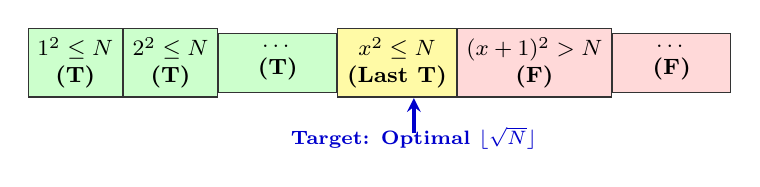
\begin{tikzpicture}[
    box/.style={rectangle, draw=black!80, font=\footnotesize, align=center, minimum height=0.75cm},
    t_box/.style={rectangle, draw=black!80, fill=green!20, font=\footnotesize\bfseries, align=center, minimum height=0.75cm},
    f_box/.style={rectangle, draw=black!80, fill=red!15, font=\footnotesize\bfseries, align=center, minimum height=0.75cm},
    arrow/.style={-stealth, very thick, blue!80!black}
]
\node[t_box, minimum width=1.1cm] (x1) at (0,0) {$1^2 \le N$\\(\textbf{T})};
\node[t_box, minimum width=1.1cm, right=0.0cm of x1] (x2) {$2^2 \le N$\\(\textbf{T})};
\node[t_box, minimum width=1.5cm, right=0.0cm of x2] (x3) {$\dots$\\(\textbf{T})};
\node[t_box, minimum width=1.4cm, fill=yellow!35, right=0.0cm of x3] (opt) {$x^2 \le N$\\(\textbf{Last T})};
\node[f_box, minimum width=1.6cm, right=0.0cm of opt] (x4) {$(x+1)^2 > N$\\(\textbf{F})};
\node[f_box, minimum width=1.5cm, right=0.0cm of x4] (x5) {$\dots$\\(\textbf{F})};

\draw[arrow] (4.3, -0.9) -- node[below, font=\scriptsize\bfseries] {Target: Optimal $\lfloor\sqrt{N}\rfloor$} (4.3, -0.45);
\end{tikzpicture}
\caption{Monotonic Boolean Predicate Transition: Locating the Boundary of the Last Valid Integer.}
\label{fig:sqrt_predicate}
\end{figure}

The problem reduces to finding the \textbf{last True value} in this monotonic range!

\subsection{Trace on Lecture Example: $N = 67$}

For $N = 67$, the integer search space is $l = 1, r = 67$. We seek $\lfloor\sqrt{67}\rfloor$:
\begin{itemize}
    \item \textbf{Pass 1:} $l = 1, r = 67, mid = 34$.
    \[
    34 \times 34 = 1156 > 67 \implies \text{Too large! Search left: } r = 33.
    \]
    \item \textbf{Pass 2:} $l = 1, r = 33, mid = 17$.
    \[
    17 \times 17 = 289 > 67 \implies \text{Too large! Search left: } r = 16.
    \]
    \item \textbf{Pass 3:} $l = 1, r = 16, mid = 8$.
    \[
    8 \times 8 = 64 \le 67 \implies \text{Valid candidate! Record } ans = 8. \text{ Search right: } l = 9.
    \]
    \item \textbf{Pass 4:} $l = 9, r = 16, mid = 12$.
    \[
    12 \times 12 = 144 > 67 \implies r = 11.
    \]
    \item \textbf{Pass 5:} $l = 9, r = 11, mid = 10$.
    \[
    10 \times 10 = 100 > 67 \implies r = 9.
    \]
    \item \textbf{Pass 6:} $l = 9, r = 9, mid = 9$.
    \[
    9 \times 9 = 81 > 67 \implies r = 8.
    \]
    \item \textbf{Termination:} Now $l = 9, r = 8 \implies l > r$. Loop halts.
\end{itemize}
The algorithm returns \textbf{$ans = 8$}, precisely matching $8^2 = 64 \le 67 < 9^2 = 81$.

\subsection{Preventing 64-bit Integer Overflow}

When $mid \approx 10^9$, computing $mid \times mid \approx 10^{18}$, which overflows a standard 32-bit signed integer (\texttt{int} max is $\approx 2 \times 10^9$). In systems code, this is mitigated by:
\begin{enumerate}
    \item Casting to 64-bit long: \verb|(long) mid * mid <= N|.
    \item Division rearrangement: \verb|mid <= N / mid| (avoiding multiplication entirely).
\end{enumerate}

\subsection{Production Java Implementation: Integer Square Root}

\begin{verbatim}
public class SquareRootSolver {
    public static int mySqrt(int N) {
        if (N <= 1) return N;

        long l = 1;
        long r = N;
        long ans = 1;

        while (l <= r) {
            long mid = l + (r - l) / 2;

            if (mid * mid <= (long) N) {
                ans = mid;    // Record valid candidate
                l = mid + 1;  // Try to find larger square
            } else {
                r = mid - 1;  // Too large, search left
            }
        }
        return (int) ans;
    }
}
\end{verbatim}

% -----------------------------------------------------------------------------
\section{Comparative Synthesis and Engineering Decision Framework}
\label{sec:synthesis}

Table~\ref{tab:comparison} synthesizes the searching paradigms examined across the lecture.

\begin{table*}[t]
\centering
\caption{Comparative Synthesis of Search Paradigms and Invariant Properties}
\label{tab:comparison}
\begin{tabular}{@{}p{1.9cm}p{2.1cm}p{2.3cm}p{2.1cm}ccp{3.6cm}@{}}
\toprule
\textbf{Search Problem} & \textbf{Input State} & \textbf{Search Space} & \textbf{Target Condition} & \textbf{Time} & \textbf{Space} & \textbf{Primary Systems Value} \\ \midrule
\textbf{Linear Search} & Unsorted / Stream & Full Array $[0 \dots N-1]$ & $A[i] == K$ & $O(N)$ & $O(1)$ & Baseline scan for small or unindexed datasets \\
\textbf{Canonical BS} & Sorted Strictly & Index Range $[0 \dots N-1]$ & $A[mid] == K$ & $O(\log N)$ & $O(1)$ & Sub-millisecond lookup in sorted index tables \\
\textbf{First Occurrence} & Sorted w/ Duplicates & Index Range $[0 \dots N-1]$ & $A[mid] == K$ (Go Left) & $O(\log N)$ & $O(1)$ & Telemetry log start boundaries, range counting \\
\textbf{Last Occurrence} & Sorted w/ Duplicates & Index Range $[0 \dots N-1]$ & $A[mid] == K$ (Go Right) & $O(\log N)$ & $O(1)$ & Telemetry log end boundaries, range counting \\
\textbf{Local Minima} & Unsorted Distinct & Internal Indices $[1 \dots N-2]$ & Valley Condition & $O(\log N)$ & $O(1)$ & Optimization in multi-modal landscapes \\
\textbf{Square Root BS} & Implicit Math Domain & Integer Range $[1 \dots N]$ & $x^2 \le N$ (Last True) & $O(\log N)$ & $O(1)$ & Discrete numerical computation without floats \\ \bottomrule
\end{tabular}
\end{table*}

\subsection{The Universal Binary Search Engineering Decision Flowchart}

When tackling any searching problem in systems engineering or technical interviews:
\begin{enumerate}
    \item \textbf{Is the input an explicit array?}
    \begin{itemize}
        \item \textbf{No:} Formulate the numerical answer range $[1 \dots \text{Max}]$ and define a boolean feasibility predicate \texttt{isPossible(mid)}. Use \textbf{Binary Search on Answer Space}.
        \item \textbf{Yes:} Proceed to evaluate array properties.
    \end{itemize}
    \item \textbf{Is the array sorted?}
    \begin{itemize}
        \item \textbf{Yes (No Duplicates):} Apply \textbf{Canonical Binary Search}.
        \item \textbf{Yes (With Duplicates):} Apply the \textbf{Answer Variable Pattern} (\texttt{r = mid - 1} for first occurrence; \texttt{l = mid + 1} for last occurrence).
        \item \textbf{No (Unsorted):} Check if the problem asks for a local extremum or peak. Use \textbf{Topographical Slope Binary Search}.
    \end{itemize}
    \item \textbf{Guard Against Boundary Hazards:}
    \begin{itemize}
        \item Midpoint overflow: always use \texttt{mid = l + (r - l) / 2}.
        \item Multiplication overflow: cast to \texttt{long} or use division.
        \item Boundary access: test indices $0$ and $N - 1$ separately before searching internal ranges.
    \end{itemize}
\end{enumerate}

% -----------------------------------------------------------------------------
\section{Conclusion}
\label{sec:conclusion}

In this research paper, we explored the algorithmic foundations of searching, demystifying the mechanisms that enable logarithmic-time performance across diverse problem topologies. We demonstrated how binary search collapses exponential search spaces through consistent halving, contrasting the newspaper scan with the dictionary lookup. We formalized pointer dynamics and midpoint overflow defenses in canonical binary search.

We resolved duplicate clustering using the Answer Variable Pattern, unlocking instantaneous range frequency calculations in database telemetry. Furthermore, we dispelled the dogma that binary search requires sorted arrays by proving how topographical valley descent guarantees finding local minima in unsorted data. Finally, we generalized binary search to implicit monotonic answer spaces, computing integer square roots through boolean predicate boundary detection. Together, these paradigms establish an exhaustive, production-grade foundation for high-performance software engineering and technical interview mastery.


\end{document}
